\section{Problem Description}
In this paper, we aim at the problem: \textit{How to achieve accuracy and scalability simultaneously in analyzing the app homology on Android Markets
?}

In order to obtain an effective app homology analysis strategy, we need to obtain an informative low-dimensional representation from the extracting CFG data. Refine such representation is a non-trivial task due to the following difficult points:
\begin{enumerate}
  \item Extracting the feature of CFG of app binary codes needs to preserve both characteristics of basic blocks and the call structure. Since CFG is a directed graph in most cases, and their corresponding vertexes have own unique features, which needs to be extracted from basic blocks. How can we carefully deal with such graph property in the representation learning process.
  %\item The ultimate goal is to train an app homology analysis system based on the learned representation of the CFG. If we can incorporate the analysis system training procedure into the representation learning process, the classifier process will indirectly interact with the original CFG via latent factors. How can we effectively fuse these two procedures together to achieving the accurate and scalability the app homology analysis?  
  \item The mass quantity of apps have the millions and billions CFG features that leads to the scalable graph match problem. Graph match essentially is a NP-problem. We need to find a practicable approach to accurately reduce CFG features. Moreover, the availability of the reducing feature should be proved theoretically and practically.
  \item The rapidly increasing novel apps cause the previous feature data that should be updated timely. Since if app samples are changed, the feature data also needs to be re-obtained. We need to find a incremental computation algorithm that just needs to compute the novel app features excluding pervious app features.   
\end{enumerate}
%\subsection{Problem Formulation}

To address those critical problems, we extract the numeric and structural features in the binary code of Android apps based on the following basic definition. %We formally define the problem of large-scale app homology analysis using the CFG extraction with basic-block feature, the first-hierarchy CFG embedding model considering the first-order call structure of CFG and the second-order call structure of CFG, and the second-hierarchy embedding tensor model based on the first-hierarchy embedding CFGs' feature vector. 
   
\textbf{Definition 1.} \emph{(CFG extraction with the basic block feature)}. We extract CFG that each vertex is with five unique feature called 5UD-CFG, is a directed graph $G=<V,E>$, where $V$ is a set of basic blocks in a function;$E \subseteq V \times V$ is a set of edges representing connections between these basic blocks. Each vertex has a unique feature with five numeric elements based on the statistical features of basic blocks. The corresponding feature of a vertex represents as a vector $v=\vec{x} =<num, ~squ, ~in, ~out, ~loop>$. $num$ is the sequence number of the basic block in the CFG, $squ$ is the number of opcodes for a basic block, $in$ is the number of calls, $out$ is the number of basic blocks that is called by other vertexes, $loop$ is the number of loops of a vertex. Each vertex has a unique weight $\omega \in \aleph$. Fig.1 (a) shows a real extracting CFG.


%\begin{figure}[hbt]
%  \center{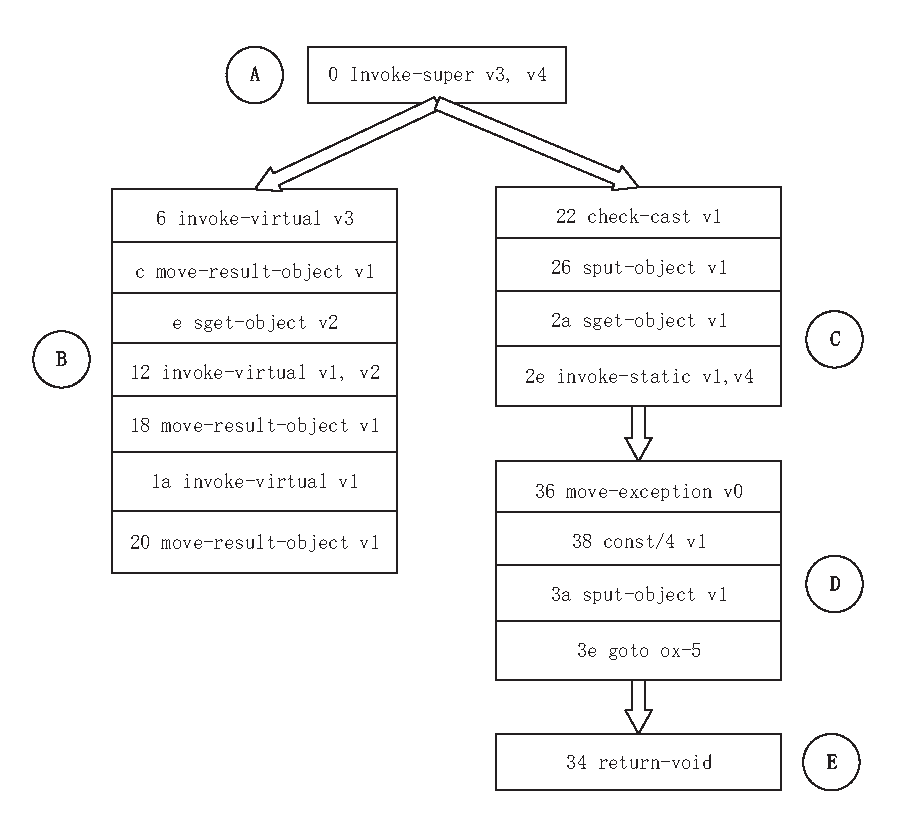
\includegraphics[width=8cm] {realcfg.eps}}
%  \caption{\label{1}  An example of real CFG}
%\end{figure}

Given a set of training CFGs $C=[c_1,~c_2,~...,~c_{N_T}]\in R^{m\times 5\times N_T}$ where $c_i \in R^{m \times 5}$ is a CFG, $m$ is the number of vertexes in a CFG, and $N_T$ is the number of all CFGs. Embedding aims to map the graph data into a low-dimensional latent space, where combines all vertexes of a CFG represented as a low-dimensional vector. As this explained, both vertex features and the graph structure are essential to be preserved.Then we define the first-hierarchy 5UD-CFG embedding model.

\textbf{Definition 2.} \emph{(First-hierarchy 5UD-CFG embedding)} Given a CFG that each vertex has five eigenvalues denoted as $G=(V, E)$, CFG embedding aims to learn a mapping function $f: \sum_1^m \vec{x_i} \mapsto y_i \in R^d$, where $d<< |V|.$ The objective of function is to distinguish the similarity between the feature of a CFG $y_i$ and the feature of another CFG $y_j$, explicitly preserve the first-order and second-order call structure of $v_i$ and $v_j$. We denote the result of first-hierarchy CFG embedding as 5UD-CFG.

We consider the \emph{first-order call structure} and the \emph{second-order call structure} to show CFG structure based on the definition of the first-hierarchy 5UD-CFG embedding.

%\begin{Definition}
\textbf{Definition 3.} \emph{(First-Order Call Structure)} The first-order call structure describes the directed pairwise structure between vertexes. For any pair of vertexes, if $l_{i,j}=1$, there exists an directed first-order call structure between the vertex $v_i$ and $v_j$.  Otherwise, the first-order call structure between the vertex $v_i$ and $v_j$ is 0.
%\end{Definition}

The first-order call structure is necessary for the CFG embedding to imply the first-order inherit or invocation between two real basic blocks in real binary codes. The result of the basic block will be directed used by the directional vertexes.

%\begin{Definition}
	\textbf{Definition 4.} \emph{(Second-Order Call Structure)} The second-order call structure between a pair of vertexes describes the call structure of neighborhoods. Let $N_u={l_{u,1}~,~...,~l_{u,|V|}}$ denote the first-order call structure between $v_u$ and other vertexes. $|V|$ is the number of neighborhoods. The second-order call structure is determined by the similarity of $N_u$ and $N_v$. 
%\end{Definition}

Intuitively, the second-order call structure assumes that if two vertexes share many common basic blocks, they may have more connections. Such an assumption has been proved reasonable in many fields \cite{TangQWZYM15}. A father basic block is most frequently called in other basic blocks.


\textbf{Definition 5.} \emph{(Second hierarchy embedding tensor model)} To represent all CFGs' features of all apps, the proposed tensor embedding model can be written as a three-order tensor model $A^{I_f*I_c*I_1}$, which $I_f, I_c$ indicate the feature vector of CFG and the number of all CFGs. For embedding CFG, $I_f=5$ and $I_c=tn$, $tn$ is the total training number of CFGs. $tn$ can be expanded with the development of apps. $I_1$ is the label of the app. Using the label $I_1$, we can partition app communities that can be easier used for the app homology analysis.
%\subsection{Problem Overview}
% the following steps: starting with a unknown app in binary code. We are searching for binaries containing the similarity functions in known app features' database. We extract the unique feature vector for each function in app. Then we handle with all extracting CFG features to achieving an effective and scalable homologous app search.

%\begin{Definition}


\section{Solution Overview}
In this section, we present the key idea of our solution to the app homology embedding problem, which can be scalable and accurate. In our approach, we show binary codes of app represented by 3TU-CFG. 

We propose the two-hierarchies embedding mapping model for the extracting CFG from app's binary codes. The two hierarchies embedding model satisfy several highlights: first, it extracts the CFG that each vertex has five unique eigenvalues. This CFG with feature is referred to the raw feature, from a decompiling binary function of app. It remains characteristics of raw binary code of app. Second, the first-hierarchy 5UD-CFG embedding is able to preserve both the \emph{first-order call structure} and the \emph{second-order call structure} between vertices of CFG. Third, the second-hierarchy tensor embedding can handle the scalable and considerable CFG feature data, say millions and billions apps' homology detection in very short time. 

The proposed methods including the following main steps, as shown in Fig. 2: 1) \emph{original CFG extraction with vertex features}, 2) \emph{5UD-CFG embedding feature vector generation}, 3) \emph{3TU-CFG tensor embedding compressing and clustering}, 4) \emph{3TU-CFG tensor embedding update}. The first step and the second step are the first-hierarchy embedding process. They aim at extracting the original control flow graph that each vertex of CFG has five eigenvalues, and embedding them into a monotonous feature vector (Section 4). The third step and the fourth step are the second-hierarchy embedding process. They use the tensor factorization learning algorithm to further embed the feature vector that is generated by the first-hierarchy embedding process to a more low-dimensionality feature vector, and this model also provide an incremental feature data update approach (Section 5). Finally, given a app, we use the KNN \cite{ChandrasekaranD18} to find its most similarity app in feature data. Since each app is decompiled into several functions, and each function is embedded into a low-dimensionality unique and accurate feature vector in two hierarchies embedding process. We can directly apply fast KNN search \cite{AntolD17} to conduct efficient matches and searches. The detailed of each steps will be discussed in the following section.

In the first-hierarchy 5UD-CFG embedding process, we show the monotonicity of 5UD-CFG feature vector, which give a high scalability and accurate. When a function changes a little, its 5UD-CFG will not change a lot. Make sure two similarity apps have a little different, and two different apps have a large different. In the second-hierarchy 3TU-CFG learning embedding process, we show the embedding reversibility and the monotonicity of 3TU-CFG, which generates a more concise embedding feature vector to monotonously map the original apps' function. The compress and clustering algorithm based on the tensor embedding model give a further significant scalability and accurate. Moreover, the tensor computations make the feature data updated easier in the second-hierarchy tensor embedding process. 

\begin{figure*}[!hbt]
   \centering
   \subfigure[]{\label{fig: 1}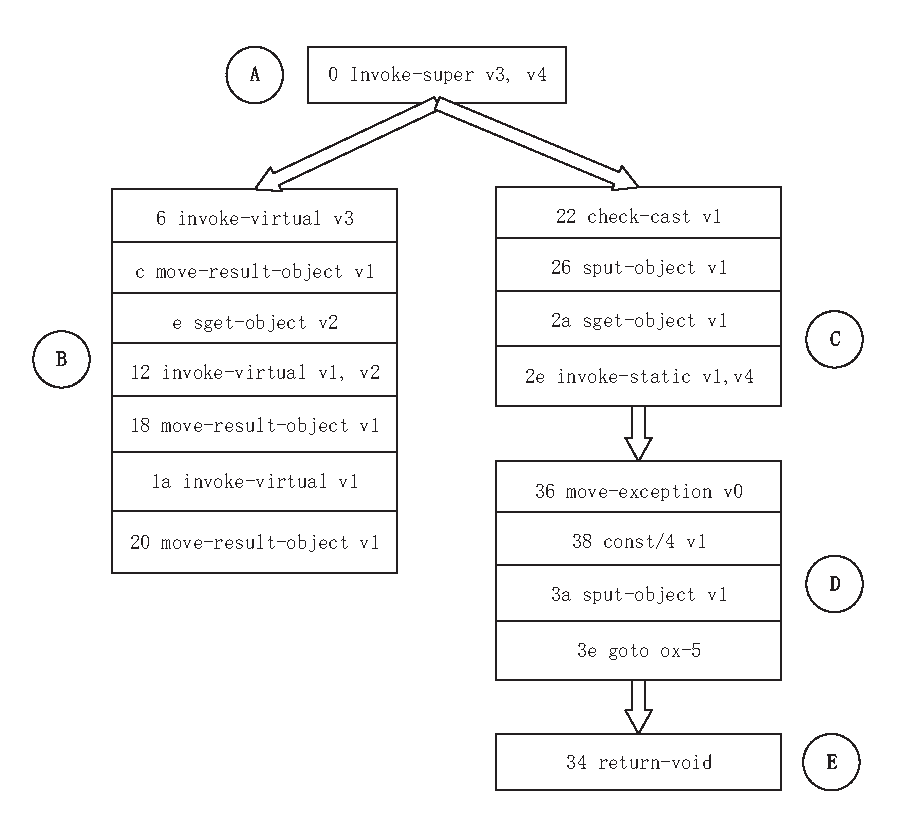
\includegraphics[width=0.30\textwidth]{realcfg.eps}}
   \hspace{0.1in}
   \subfigure[]{\label{fig: 2}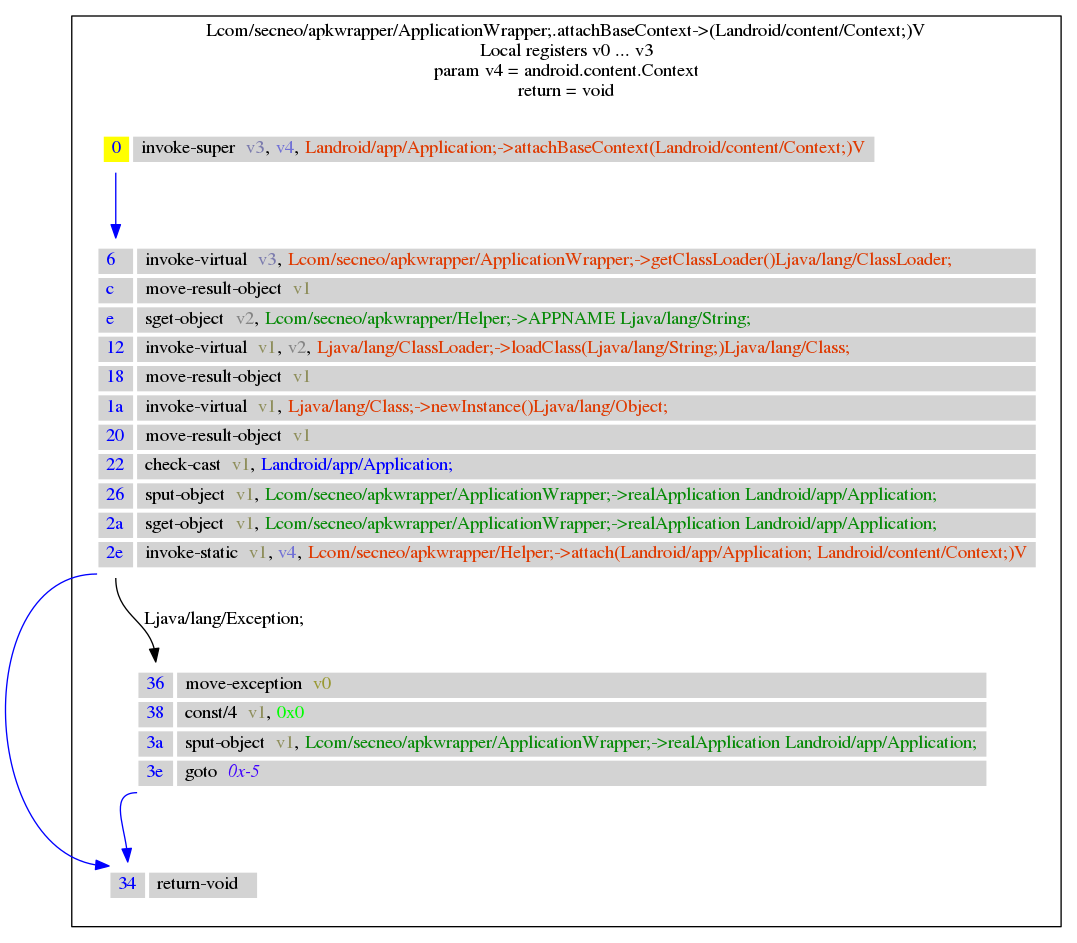
\includegraphics[width=0.30\textwidth]{cfgexample.png}} \hspace{0.1in}
   \subfigure[]{\label{fig: 3}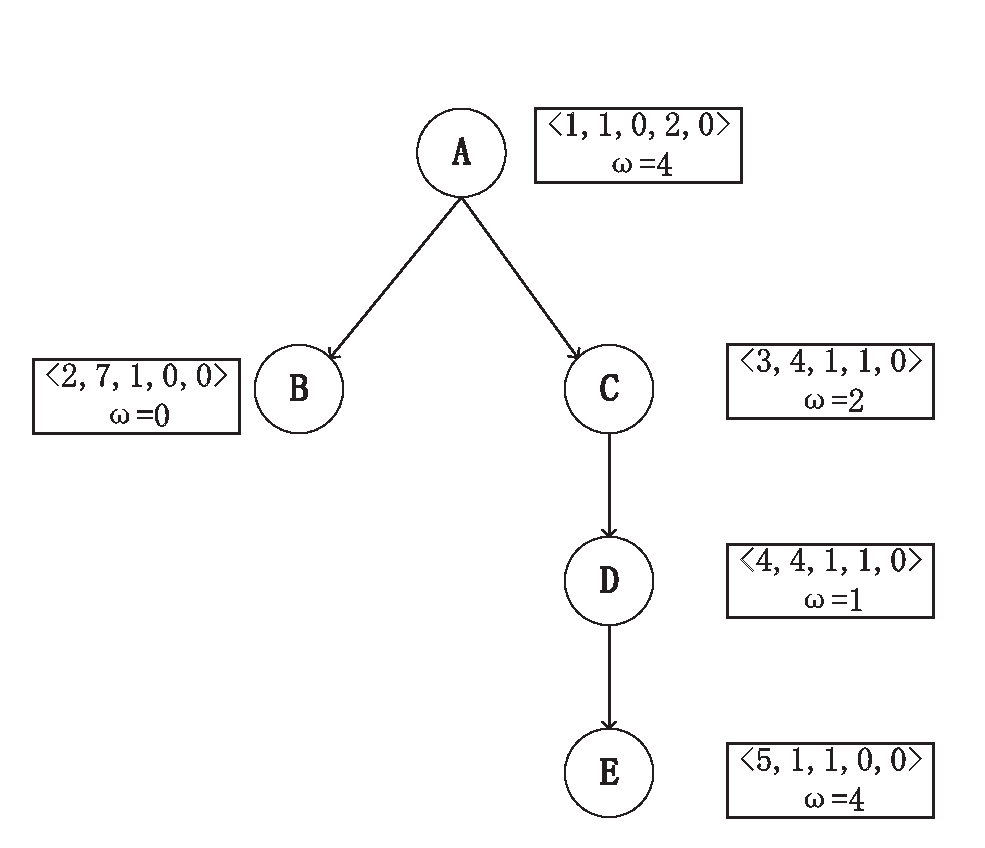
\includegraphics[width=0.30\textwidth]{feature.eps}}\\
   \caption{(a) shows an example of real CFG; (b) shows extracting CFG with the basic block; (c) shows an example of CFG with embedding feature; (a) is used in this Section 3, (b) and (c) are used in Section 5. }
   \vspace{-3 mm}
   \end{figure*}
   
   \begin{figure*}[!hbt]
  \center{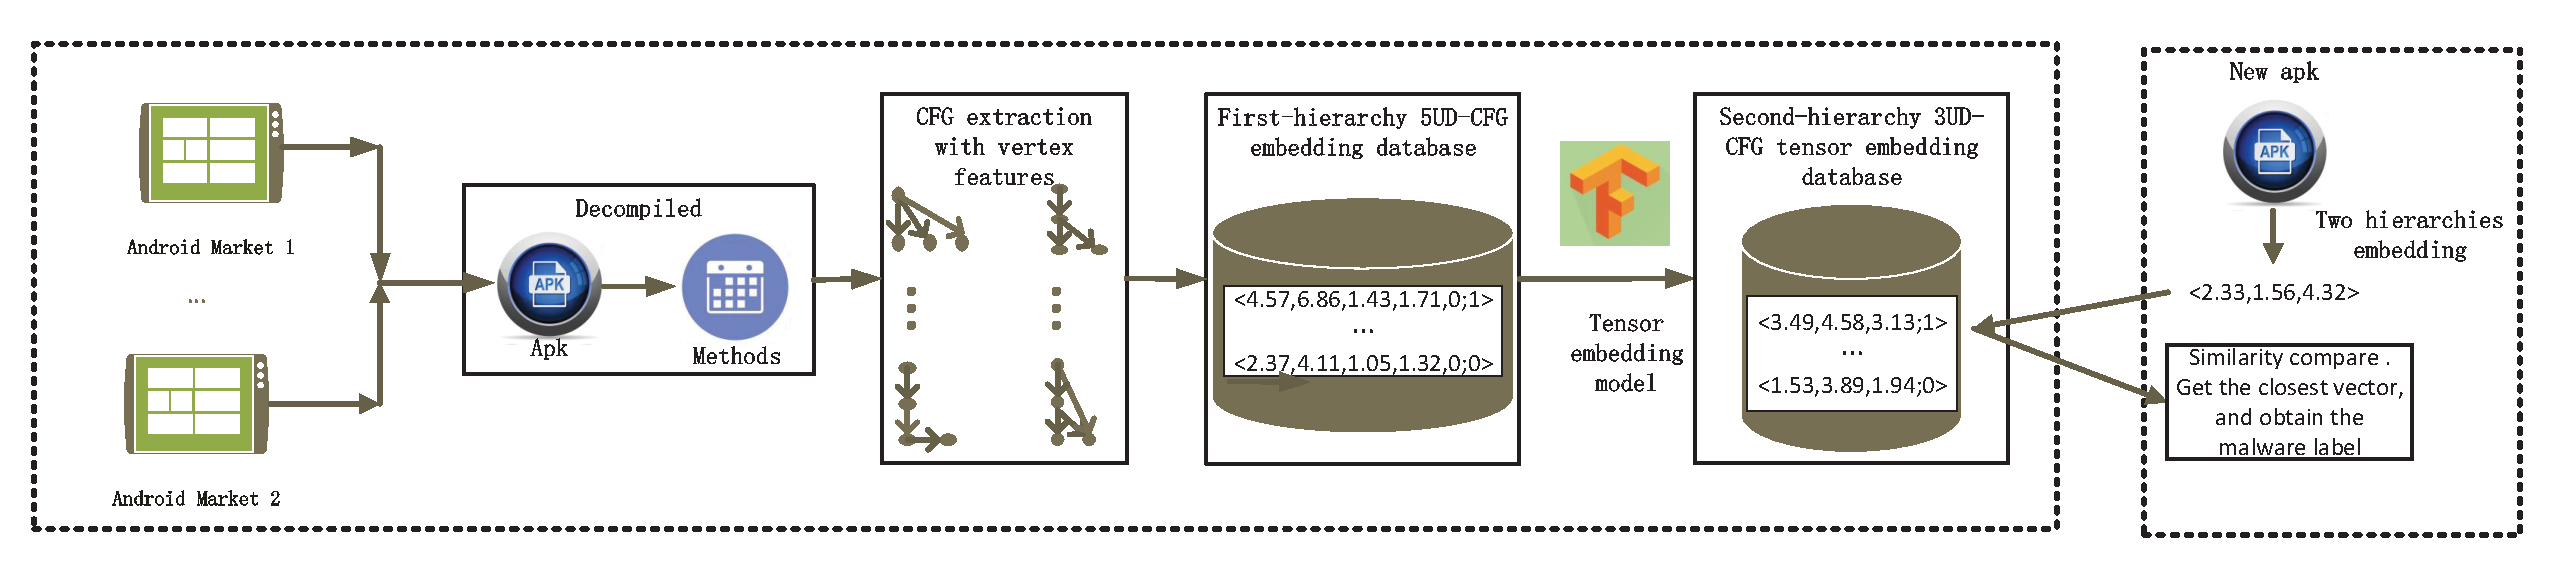
\includegraphics[width=18cm] {overview.eps}}
  \caption{Overview}
\end{figure*}
                                                                                                                                                                                                                                                                                                                                                                                                                                                                                                                                                                                                                                                                                                                                                                                                                                                                                                                                                                                                                                                                                                                                                                                                                                                                                                                                                                                                                                                                                                                                                                  